% SOURCE : http://forum.mathematex.net/latex-f6/tableau-de-signes-complexe-t11291.html#p110019

\documentclass{article}
	\usepackage[utf8]{inputenc}
	\usepackage[T1]{fontenc}
	\usepackage{lmodern}
	\usepackage{tkz-tab}
	\usepackage{amsmath,fullpage}

	\parindent=0pt


\begin{document}

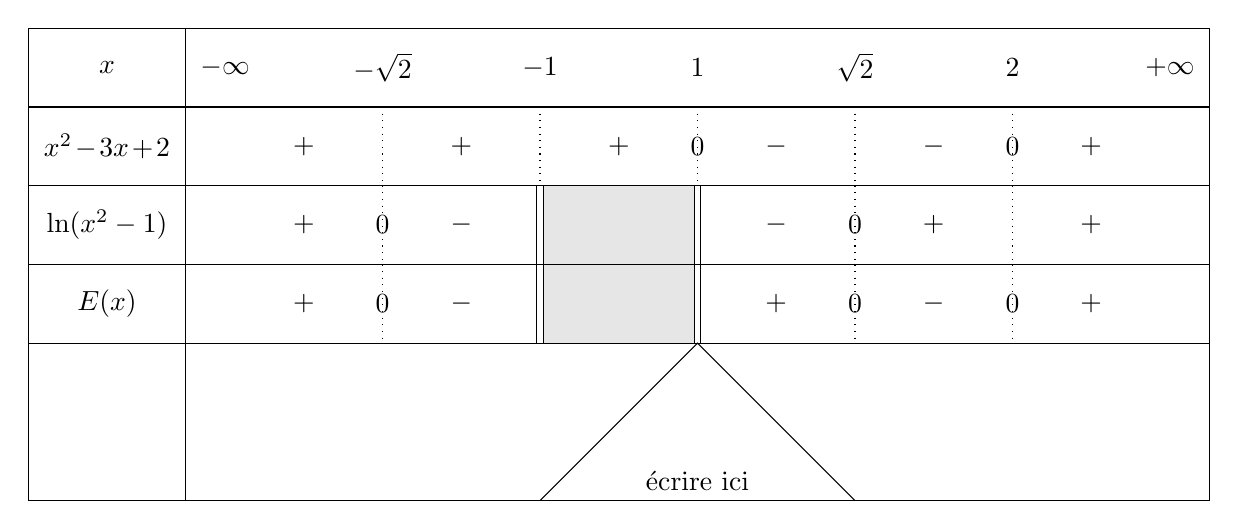
\begin{tikzpicture}
	\tkzTabSetup[
		doubledistance = 2pt,
		tstyle = dotted,
		hopacity = .2,
		hcolor = red!50!black
	]
	\tkzTabInit[lgt=2,espcl=2]{%
		$x$         /1,
		$x^2-3x+2$   /1,
		$\ln (x^2-1)$/1,
		$E(x)$       /1,
		/2 %
	}%
	{$-\infty$ ,$-\sqrt{2}$, $-1$ , $1$ ,$\sqrt{2}$ , $2$ , $+\infty$}%
	\tkzTabLine{ , + , t , + , t , + , z , - , t , - , z , + , }
	\tkzTabLine{ , + , z , - , d , h , d , - , z , + , t , + , }
	\tkzTabLine{ , + , z , - , d , h , d , +  ,z , - , z , + , }
	\draw(N35)--(N44)--(N55);
	\node[above] at (N45) {écrire ici};
\end{tikzpicture}

\end{document}
